\documentclass[a4paper]{article}
\usepackage[italian]{babel}
\usepackage[style=ieee,backend=biber]{biblatex} \addbibresource{bibliography.bib}
\usepackage{csquotes}
\usepackage{hyperref}
\usepackage{algorithm}
\usepackage{algpseudocode}
\usepackage[table]{xcolor}
\usepackage{minted}
\usepackage{amsmath}
\usepackage{listings}
\usepackage{xcolor}
\usepackage{graphicx}
\usepackage{hyperref}
\DeclareMathOperator{\lcm}{lcm}

\lstset{
    language=C++,
    basicstyle=\ttfamily\small,
    keywordstyle=\color{blue},
    commentstyle=\color{gray},
    stringstyle=\color{red},
    numbers=left,
    numberstyle=\tiny\color{gray},
    stepnumber=1,
    numbersep=10pt,
    tabsize=2,
    showspaces=false,
    showstringspaces=false,
    breaklines=true,
    frame=single,
    backgroundcolor=\color{lightgray},
    captionpos=b
}

\title{Report PHPC}
\author{Pierluigi Supino \and Rodolfo Diana \and Salvatore Di Gennaro}

\begin{document}

\maketitle
\tableofcontents

\section{Introduzione}

Sviluppare un’applicazione per il prodotto tra matrici su cluster multi-nodo e multi-GPU per nodo (MPI + CUDA, attraverso SLURM). All’interno di questa applicazione devono essere possibili entrambe le seguenti:
\begin{enumerate}
    \item utilizzare kernel originali per i calcoli sulla GPU;
    \item utilizzare funzioni della libreria cuBLAS in alternativa a quelle originali.
\end{enumerate}

\section{Implementazione}
In un ambiente multi-nodo e multi-GPU, il prodotto tra matrici può essere articolato in due livelli distinti ma interconnessi.

A un livello più alto è necessario decomporre il problema a livello globale, ovvero suddividere le matrici da moltiplicare in blocchi che possano essere assegnati in modo efficiente ai diversi nodi del cluster, tenendo conto del bilanciamento del carico, della minimizzazione della comunicazione tra nodi e dell'architettura del sistema.

A un livello più basso, invece, entra in gioco l’effettiva esecuzione del prodotto tra i blocchi locali di matrici all’interno di ciascun nodo, sfruttando le GPU a disposizione. Volendo si potrebbe suddividere questo livello in ulteriori due parti: il partizionamento delle matrice tra le diverse GPU e l'esecuzione dei calcoli reali.

\subsection{Processi}
Il prodotto tra matrici viene eseguito a livello di processi tramite SUMMA (Scalable Universal Matrix Multiplication Algorithm)\cite{SUMMA}.

Disponiamo i diversi processi una griglia logica bidimensionale $r \times c$ e sia $l=\lcm(r, c)$. e assegniamo loro delle sottomatrici nel seguente modo:
% suddivisione
$$
    A=
    \begin{pmatrix}
        A_{00}     & \cdots & A_{0(c-1)}     \\
        \vdots     & \ddots & \vdots         \\
        A_{(r-1)0} & \cdots & A_{(r-1)(c-1)}
    \end{pmatrix}
$$

$$
    B=
    \begin{pmatrix}
        A_{00}     & \cdots & A_{0(c-1)}     \\
        \vdots     & \ddots & \vdots         \\
        A_{(r-1)0} & \cdots & A_{(r-1)(c-1)}
    \end{pmatrix}
$$

$$
    C_{ij}=\sum_{l=0}^{c-1}A_{ij}B_{ij}
$$

Nel nostro algoritmo si suppone che le matrici in input siano allocate come array contigui \textit{row-major} di dimensione $n^2$ e che contengano già al loro interno (almeno) i dati del blocco assegnato al processo chiamante.
L'algoritmo funziona a fasi, in cui per ognuna i processi collaborano per combinare blocchi specifici delle matrici $A$ e $B$. Ogni riga di processi condivide tra sé il blocco di $A$ rilevante per quella fase, mentre ogni colonna fa lo stesso con un blocco di $B$. Questo avviene tramite un'operazione di broadcast dello standard di comunicazione \textit{Message Passing Interface} (MPI)\footnote{\url{https://docs.open-mpi.org/en/v5.0.x/man-openmpi/man3/MPI_Bcast.3.html}}. Sono stati creati dei tipi derivati appositi per tenere in considerazione gli spazi di memoria che intercorrono tra una riga e l'altra dei blocchi da inviare\footnote{\url{https://docs.open-mpi.org/en/v5.0.x/man-openmpi/man3/MPI_Type_vector.3.html}}.

\begin{table}[h]
    \center
    \begin{tabular}{|c|c|c|c|}
        \hline
        \cellcolor{yellow}0 & \cellcolor{yellow}1 & 2  & 3  \\ \hline
        \cellcolor{yellow}4 & \cellcolor{yellow}5 & 6  & 7  \\ \hline
        8                   & 9                   & 10 & 11 \\ \hline
        12                  & 13                  & 14 & 15 \\ \hline
    \end{tabular}
    \begin{tabular}{|c|c|c|c|c|c|c|c|c}
        \hline
        \cellcolor{yellow}0 & \cellcolor{yellow}1 & 2 & 3 & \cellcolor{yellow}4 & \cellcolor{yellow}5 & 6 & 7 & \dots \\ \hline
    \end{tabular}
    % \caption{Rappresentazione in memoria di una matrice \textit{row-major}}
\end{table}

Una volta ricevuti i blocchi necessari, ogni processo può calcolare una parte del prodotto parziale della matrice $C$, sommando il risultato a quello già accumulato. Ripetendo questa operazione per un numero di fasi pari alla dimensione della griglia, alla fine ogni processo avrà calcolato il suo blocco completo di $C$.

\begin{algorithm}[h]
    \caption{SUMMA}
    \begin{algorithmic}
        \State $C_{ij} \gets 0$
        \For{$i \gets 0$ \textbf{to} $k - 1$}
        \State broadcast $A_{ij}$ within my row
        \State broadcast $B_{ij}$ within my column
        \State $C_{ij} \gets C_{ij} + AB$
        \EndFor
    \end{algorithmic}
\end{algorithm}

Eseguite tutte le operazioni, l'ultimo passaggio consiste nel ricomporre le diverse sottomatrici dai vari processi. In generale sono disponibili diversi approcci a seconda di come sia necessario il risultato. In questo caso è stato deciso, per semplicità, che solo il processo 0 debba avere la matrice finale completa. Non è stata implementata una particolare gestione degli errori per evitare overhead nelle misurazioni dei tempi.

\subsection{GPU}
\subsubsection{Multi-GPU}
Per sfruttare al massimo le risorse disponibili, è stato necessario sviluppare un sistema che permettesse la suddivisione del lavoro su più GPU presenti nella macchina.

L'obiettivo consiste nel sovrapporre quanto più possibile il lavoro svolto dalle diverse GPU ed evitare conflitti di memoria che dovrebbero essere serializzati, in particolare la scrittura sulla matrice $C$. Un'idea naturale è partizionare quest'ultima in modo che ogni device possa eseguire le operazioni in uno spazio separato dagli altri.
Una suddivisione semplice ma funzionale per qualsiasi numero di GPU è quella per colonne: ogni GPU effettua quindi il prodotto tra la matrice A e la ``colonna'' assegnata della matrice B.

% $$
%     B=
%     \begin{pmatrix}
%               &        &           \\
%         B_{0} & \cdots & B_{n - 1} \\
%               &        &
%     \end{pmatrix}\\
%     C=
%     \begin{pmatrix}
%               &        &           \\
%         C_{0} & \cdots & C_{n - 1} \\
%               &        &
%     \end{pmatrix}
% $$

% $$
%     C^i = \sum_{k=0}^{n-1} A_{k}B^i
% $$

Questo meccanismo implica, ovviamente, che l'host debba essere in grado di avviare l'esecuzione su più GPU senza dover attendere prima il completamento di una di esse.
Un metodo sicuramente valido è creare diversi thread a livello di processo, ognuno dei quali gestisca un determinato device.
Tuttavia, CUDA offre anche varianti asincrone delle diverse funzioni e la possibilità di gestirle tramite \textit{stream}, ovvero code di operazioni da eseguire in sequenza.

% TODO: aggiungere pseudocodice
\begin{algorithm}[h]
    \caption{MultiGPU}
    \begin{algorithmic}
        % \State $C_{ij} \gets 0$
        \For{$i \gets 0$ \textbf{to} $n - 1$}
        \State cudaStreamCreate($s_i$)
        \State cudaMallocAsync($dev_a$)
        \State $C_i \gets cudaMemcpy()$
        \State $C_{ij} \gets C_{ij} + AB$
        \EndFor
        \For{$i \gets 0$ \textbf{to} $n - 1$}
        \State wait stream $i$
        \State destroy stream $i$
        \EndFor
    \end{algorithmic}
\end{algorithm}

\subsubsection{Kernel}

La moltiplicazione tra una matrice M $(I\times{J})$ e una matrice N $(J\times{K})$ produce una matrice P $(I\times{K})$. Ognuno degli elementi della matrice $P$ è il prodotto scalare tra una riga di $M$ e una colonna di $N$. Riferendoci agli elementi di $P$ con $P_{\text{row}, \text{col}}$ avremo:

\[
    P_{\text{row}, \text{col}} = \sum_{k=0}^{\text{Width}-1} M_{\text{row}, k} \cdot N_{k, \text{col}}
\]

Ovvero per calcolare ad esempio l'elemento $P_{1, 5}$:

\[
    P_{1,5} = M_{1,0} \cdot N_{0,5} + M_{1,1} \cdot N_{1,5} + M_{1,2} \cdot N_{2,5} + \ldots + M_{1,\text{width}-1} \cdot N_{\text{width}-1,5}
\]

Per implementare la moltiplicazione tra matrici usando CUDA, possiamo mappare i thread nelle griglia agli elementi della matrice di output $P$. In questo modo, ogni thread sarà responsabile del calcolo di un elemento di $P$. Gli indici di colonna per gli elemendi di $P$ sarano:

\[
    \begin{aligned}
        \text{row} & = \text{blockIdx.y} \times \text{blockDim.y} + \text{threadIdx.y} \\
        \text{col} & = \text{blockIdx.x} \times \text{blockDim.x} + \text{threadIdx.x}
    \end{aligned}
\]

Con questo mapping uno a uno il nostro kernel sarà:

\begin{lstlisting}[caption={Kernel CUDA con memoria globale}, label={lst:1}]
__global__ void MatrixMulKernel(float* M, float* N,
                                float* P, int Width) {
    int row = blockIdx.y*blockDim.y+threadIdx.y;
    int col = blockIdx.x*blockDim.x+threadIdx.x;
    if ((row < Width) && (col < Width)) {
        float Pvalue = 0;
        for (int k = 0; k < Width; ++k) {
            Pvalue += M[row*Width+k]*N[k*Width+col];
        }
        P[row*Width+col] = Pvalue;
    }
}
\end{lstlisting}

\newpage

La Figura~\ref{fig:1}, mostra come viene suddivisa la matrice $P$ ($4\times{4}$) in una griglia di blocchi $2\times{2}$ con blocchi $2\times{2}$. Mentre la Figura~\ref{fig:2} ne mostra una parte dell'esecuzione.

\begin{figure}[H]
    \centering
    \begin{minipage}[b]{0.45\textwidth}
        \centering
        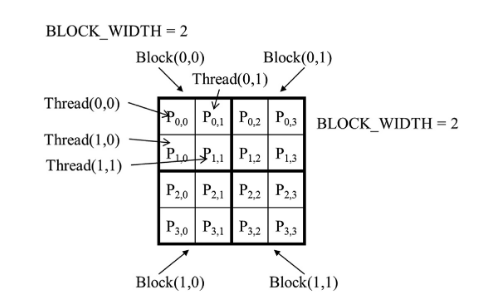
\includegraphics[width=\textwidth]{imgs/matrix_division.png}
        \caption{Divisione della matrice in una griglia di blocchi}
        \label{fig:1}
    \end{minipage}
    \hspace{0.05\textwidth}
    \begin{minipage}[b]{0.45\textwidth}
        \centering
        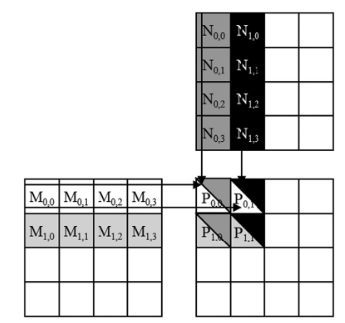
\includegraphics[width=\textwidth]{imgs/execution1.png}
        \caption{Esecuzione del kernel}
        \label{fig:2}
    \end{minipage}
\end{figure}

Questo è un approccio basilare con ampi margini di miglioramento, infatti in un contesto CUDA è fondamentale ragionare tenendo in considerazione le differenti prestazioni delle differenti memorie: la memoria globale è grande ma lenta di controparte la memoria condivisa è piccola ma veloce. Una stategia decisamente migliore rispeetto a quella presentata in precedenza è quella di partizionare i dati in sottoinsiemi chiamati \textit{tiles} in modo tale che ognuna di essa entri nella memoria condivisa con un importante vincolo, la computazione del kernel sulla singola tile può essere fatta indipendentemente dalle altre. Tornando all' esempio precedente mostriamo gli accessi alla memoria globale generati dal'esempio in Figura~\ref{fig:2}:

\begin{figure}[H]
    \centering
    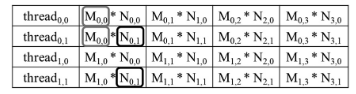
\includegraphics[width=0.6\textwidth]{imgs/memory_access.png}
    \caption{Accessi alla memoria globale}
    \label{fig:3}
\end{figure}

Nella Figura~\ref{fig:3} possiamo notare come gli stessi elementi vengano letti dalla lenta memoria globale in diversi step dell'esecuzione. In generale data la dimensione dei blocchi $width\times{width}$ ogni elemento delle matrici $M$ ed $N$ è letto dalla memoria globale $width$ volte. L'idea è quindi quella di far collaborare i threads per caricare in memoria condivisa anticipatamente tutti i dati per poi procedere allo sviluppo dei calcoli cosi facendo stiamo riducendo di $\frac{1}{width}$ gli accessi alla memoria. La Figura~\ref{fig:1} mostra gli accessi alla memoria per questo approccio.

\begin{figure}[H]
    \centering
    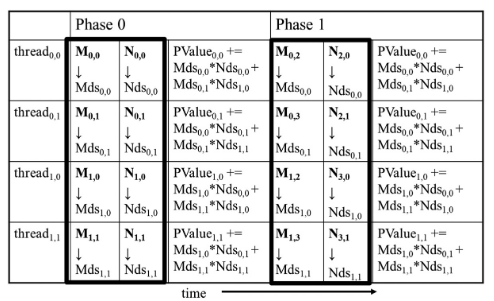
\includegraphics[width=0.6\textwidth]{imgs/memory_access1.png}
    \caption{Accessi alla memoria globale e caricamento in memoria condivisa}
    \label{fig:4}
\end{figure}

Il Listing~\ref{lst:2} mostra il kernel con l'approccio tiling e memoria condivisa.

\begin{lstlisting}[caption={Kernel CUDA con tiling e memoria condivisa}, label={lst:2}]
#define TILE_WIDTH 16
__global__ void matrixMulKernel(float* M, float* N, float* P, int Width) {
    __shared__ float Mds[TILE_WIDTH][TILE_WIDTH];
    __shared__ float Nds[TILE_WIDTH][TILE_WIDTH];

    int bx = blockIdx.x; int by = blockIdx.y;
    int tx = threadIdx.x; int ty = threadIdx.y;

    int Row = by * TILE_WIDTH + ty;
    int Col = bx * TILE_WIDTH + tx;

    float Pvalue = 0;
    for (int ph = 0; ph < Width/TILE_WIDTH; ++ph) {
        Mds[ty][tx] = M[Row*Width + ph*TILE_WIDTH + tx];
        Nds[ty][tx] = N[(ph*TILE_WIDTH + ty)*Width + Col];
        __syncthreads();

        for (int k = 0; k < TILE_WIDTH; ++k)
            Pvalue += Mds[ty][k] * Nds[k][tx];
        __syncthreads();
    }
    P[Row*Width + Col] = Pvalue;
}
\end{lstlisting}

TODO kernel con grid stride loop

\subsubsection{cuBLAS}
In alternativa a scrivere le proprie funzioni per il calcolo tra matrici, è disponibile la libreria cuBLAS sviluppata da NVIDIA che fornisce una versione ottimizzata per GPU delle routine BLAS (Basic Linear Algebra Subprograms), una serie standard di operazioni fondamentali in algebra lineare\footnote{\url{https://netlib.org/blas/}}. Sono inoltre disponibili diverse estensioni, tra cui cuBLASXt progettata per sfruttare più GPU contemporaneamente. Non sono necessari preparativi particolari, dato che si occupa autonomamente di allocare la memoria tra le GPU designate, distribuire il carico di lavoro tra di loro e infine recuperare i risultati sull'host\footnote{\url{https://docs.nvidia.com/cuda/cublas/index.html\#using-the-cublasxt-api}}.

Una nota tecnica riguarda la discrepanza tra l'ordine in memoria delle matrici: cuBLAS, per rimanere conforme alle specifiche Fortran di BLAS, si aspetta che i valori siano disposti per \textit{column-major} mentre lo standard nel C è \textit{row-major}. Fortunatamente, è possibile evitare operazioni di memoria aggiuntive il fatto che i due metodi sono le rispettive trasposte e calcolare
$$
    \mathbf{C}^T=(\mathbf{B}\mathbf{A})^T
$$
Il risultato sarà quindi salvato in una matrice column-major e che quindi corrisponderà al risultato cercato leggendolo in row-major.

\section{Analisi}

\subsection{Configurazione dei test}

\subsection{Analisi delle misurazioni}

\subsection{NVIDIA Nsight Compute}

\section{Esplorazione di NNCL}

\subsection{Introduzione}

\subsection{Possibili implementazioni}

\printbibliography

\end{document}